% ============================================================
% SECTION 3: MODEL PROPOSAL
% Paste this into StudyCoach_Report2.tex, replacing Section 3
% Assumes: \usepackage{booktabs}, \usepackage{graphicx}, \usepackage{hyperref}
% Place SVG-exported PNGs in your figures/ directory
% ============================================================

\section{Model Proposal (1 Page)}

% Include architecture diagram(s) — place your SVGs/PNGs in figures/
\begin{figure}[t]
\centering
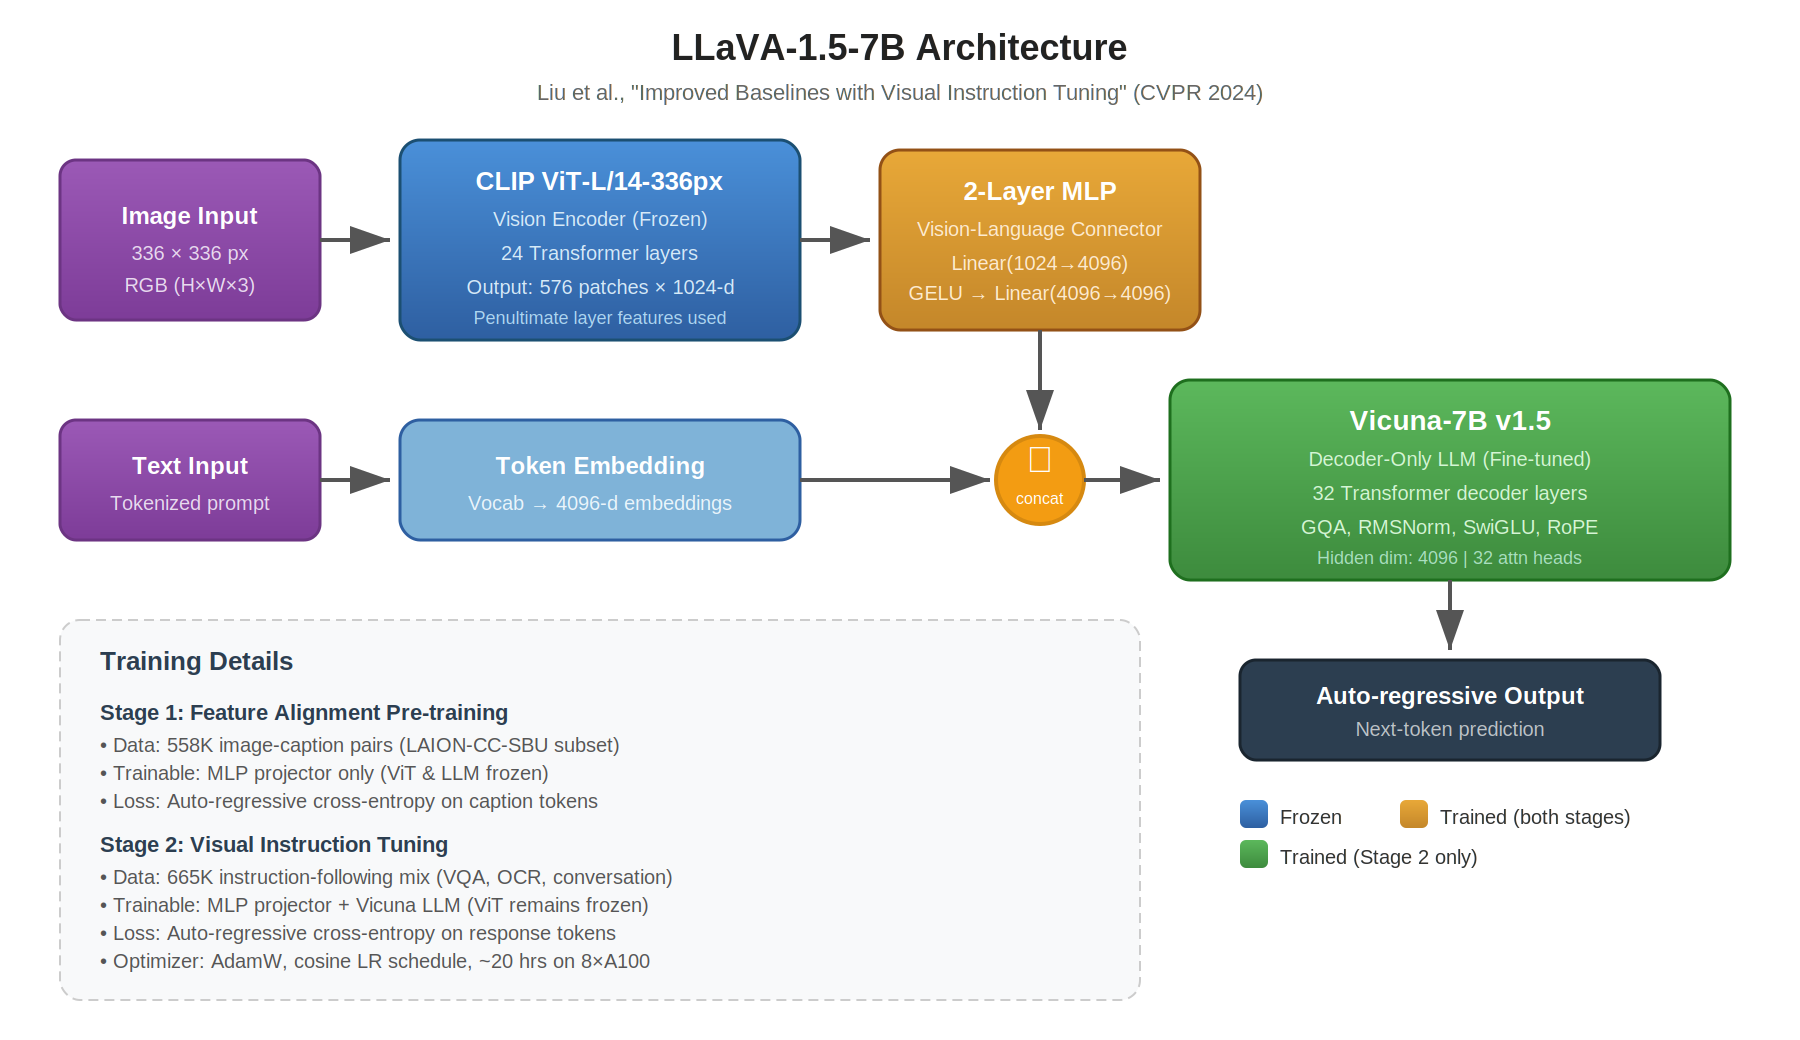
\includegraphics[width=0.95\textwidth]{figures/llava_architecture.png}
\caption{LLaVA-1.5-7B architecture: frozen CLIP ViT-L/14 $\rightarrow$ 2-layer MLP $\rightarrow$ Vicuna-7B.}
\label{fig:llava-arch}
\end{figure}

\begin{figure}[t]
\centering
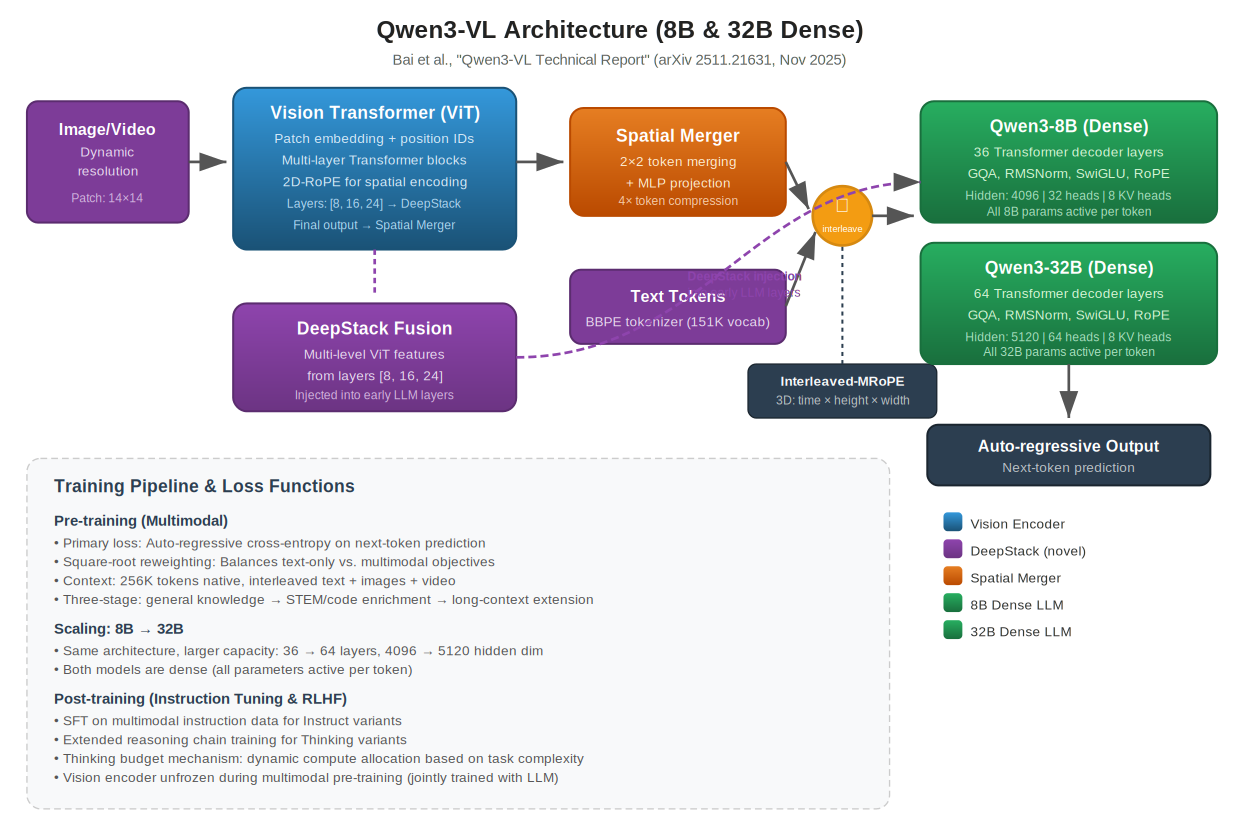
\includegraphics[width=0.95\textwidth]{figures/qwen3vl_architecture.png}
\caption{Qwen3-VL architecture (8B and 32B dense): jointly-trained ViT with DeepStack $\rightarrow$ Spatial Merger $\rightarrow$ Qwen3 decoder with Interleaved-MRoPE.}
\label{fig:qwen-arch}
\end{figure}

\subsection{\points{1.5} Overall Model Structure}

Our Study Coach system evaluates student answers to figure-grounded questions from scientific papers. We selected three vision-language models (VLMs) that share a common architecture: a \textbf{vision encoder} that converts figure images into patch-level features, a \textbf{cross-modal connector} that projects visual features into the language model's embedding space, and a \textbf{decoder-only LLM} that auto-regressively generates the verdict, error category, and coaching feedback.

The models differ in their approach to \textbf{transference}---transferring knowledge between modalities \citep{Liang-foundations-2024}. LLaVA-1.5 uses \emph{cross-modal transfer} from a frozen CLIP encoder, while Qwen3-VL uses \emph{co-learning} via joint encoder-decoder training. Our 8B baseline results show this distinction matters: text\_only verdict accuracy (56\%) outperformed multimodal (48\%), suggesting transferred visual representations can introduce noise at 8B scale---though they substantially improve explanation quality (80\% vs.\ 40\% human match rate).

\subsection{\points{1} Encoders}

\textbf{LLaVA-1.5-7B} uses CLIP ViT-L/14 at fixed $336{\times}336$ resolution (576 patches $\times$ 1024-d, penultimate layer features). The encoder is \textbf{completely frozen}---a pure cross-modal transfer approach where CLIP's web-scale contrastive features are projected into the LLM's space without adaptation. This limits scientific figure understanding to what CLIP learned from general image-text pairs, which may not support the fine-grained numerical extraction our task demands (e.g., distinguishing a bar at 84.6\% from 89\%).

\textbf{Qwen3-VL (8B and 32B)} uses a ViT with \textbf{dynamic resolution} (variable patch counts preserving native aspect ratio) and \textbf{2D-RoPE} encoding spatial position within the ViT. This encoder is \textbf{jointly trained} with the LLM---a co-learning approach where visual and linguistic representations co-adapt, directly addressing the transference challenge. Our dataset's visual heterogeneity (tables 44.3\%, plots 28.1\%, schematics 17.4\%) creates a \textbf{quantification} challenge \citep{Liang-foundations-2024}: each figure type encodes information differently, and our H4 results confirm this---tables are easiest for verdict accuracy (51.4\% avg at 8B) but hardest for feedback quality (6.4\% match), while schematics benefit most from visual context (+9.4pp verdict, +25.0pp feedback at 8B).

\textbf{Alternative: SigLIP} replaces CLIP's softmax contrastive loss with sigmoid-based binary classification, offering better-calibrated visual-text matching scores potentially useful for partial-correctness detection. All three models process text through their LLM's token embedding layer; Qwen3-VL's 151K-token BPE vocabulary provides finer-grained tokenization of scientific terminology than LLaVA's 32K vocabulary.

\subsection{\points{1} Decoders}

\textbf{LLaVA-1.5-7B} uses Vicuna-7B v1.5 (LLaMA-2 fine-tune; 32 layers, 4096-d, GQA, SwiGLU, 1D RoPE, ${\sim}$4K context). Visual tokens from the 2-layer MLP projector (GELU, 1024$\rightarrow$4096) are concatenated with text tokens before the first layer---a shallow alignment creating a large modality gap.

\textbf{Qwen3-VL-8B} uses a 36-layer Qwen3 decoder (4096-d, 32 attention heads, 8 KV heads via GQA) with \textbf{Interleaved-MRoPE} encoding three spatial-temporal dimensions (24-d temporal, 20-d height, 20-d width), enabling the decoder to ground spatial claims to specific figure regions. Its \textbf{DeepStack} mechanism \citep{ge2024deepstack} injects multi-level ViT features from layers 8, 16, and 24 into early LLM layers, creating multiple transference pathways that preserve low-level visual details (character shapes for OCR, edges for trend detection). The 256K context window accommodates full paper context.

\textbf{Qwen3-VL-32B} scales the same architecture to 64 layers with 5120-d hidden dimensions, 64 attention heads, and 8 KV heads (32.8B total parameters). Our scaling experiments confirm the larger decoder provides substantially greater cross-modal reasoning capacity: multimodal feedback match improved from 6\% to 20\% (LLM judge, $n{=}50$), schematics' visual context benefit doubled from +9.4pp to +18.8pp for verdict accuracy, and visual context began \emph{helping} conceptual error detection (+2.4pp) whereas at 8B it hurt all error types. The shared DeepStack and MRoPE mechanisms mean both Qwen3-VL models use the same multi-level fusion strategy, with the 32B's additional depth providing more layers for integrating transferred visual information.

Our finding that auto metrics (${\sim}$0.30 F1 across all scenarios at both scales) failed to capture the 2$\times$ difference in feedback quality revealed by human evaluation (multimodal 80\% vs.\ text\_only 40\% at 8B) demonstrates a \textbf{quantification} failure \citep{Liang-foundations-2024}: standard NLP metrics cannot quantify cross-modal reasoning quality, motivating our LLM-as-judge and manual evaluation approach.

\subsection{\points{1} Loss Functions}

\textbf{Primary: Auto-regressive cross-entropy.} All three models use $\mathcal{L} = -\sum_i \log P(t_i \mid V, t_1, \ldots, t_{i-1})$ over response tokens only. We do not modify this for our inference-only experiments.

\textbf{Auxiliary 1: CLIP Contrastive Loss (InfoNCE).} This symmetric contrastive loss shaped LLaVA's frozen encoder features via image-text matching. The resulting coarse-grained alignment may explain why visual input hurts verdict accuracy for factual errors ($-$21.2pp at 8B)---CLIP features support semantic matching but not the precise numerical extraction needed to verify specific claims. Factual errors require \emph{non-redundant cross-modal interaction} \citep{Liang-foundations-2024}: the correct value exists only in the visual modality, the claimed value only in text, and the model must extract and compare both precisely.

\textbf{Auxiliary 2: Square-Root Reweighting.} Qwen3-VL scales multimodal sample loss by $\sqrt{N_\text{text}/N_\text{multimodal}}$ during pre-training, preventing degradation on text understanding while learning visual grounding. Our results confirm this dual capability matters: visual context helps all error types for feedback quality (factual +21.2pp, conceptual +31.7pp, omission +33.3pp at 8B) even while hurting verdict accuracy.

\textbf{Auxiliary 3 (Proposed): Verdict-Classification Head.} For future fine-tuning on SPIQA+, we propose extracting the hidden state at the verdict token position and passing it through a lightweight 3-class classification head supervised with cross-entropy against ground-truth labels. This would provide direct supervisory signal for the detection task (H1) alongside the generative explanation loss.

% Architecture Summary Table
\begin{table}[t]
\centering
\caption{Architecture summary of the three models used for SPIQA+ inference.}
\label{tab:arch-summary}
\small
\begin{tabular}{@{}lccc@{}}
\toprule
\textbf{Component} & \textbf{LLaVA-1.5-7B} & \textbf{Qwen3-VL-8B} & \textbf{Qwen3-VL-32B} \\
\midrule
Vision Encoder & CLIP ViT-L/14 (frozen) & ViT + 2D-RoPE (joint) & ViT + 2D-RoPE (joint) \\
Cross-Modal Bridge & 2-layer MLP & Spatial Merger + DeepStack & Spatial Merger + DeepStack \\
LLM Backbone & Vicuna-7B (32L, 4096-d) & Qwen3-8B (36L, 4096-d) & Qwen3-32B (64L, 5120-d) \\
Attention & GQA (32h) & GQA (32h / 8kv) & GQA (64h / 8kv) \\
Position Encoding & 1D RoPE & Interleaved 3D MRoPE & Interleaved 3D MRoPE \\
Context Length & ${\sim}$4K tokens & 256K tokens & 256K tokens \\
Transference & Cross-modal (frozen) & Co-learning (joint) & Co-learning (joint) \\
Loss Functions & AR cross-entropy & AR CE + $\sqrt{}$ reweight & AR CE + $\sqrt{}$ reweight \\
\bottomrule
\end{tabular}
\end{table}
